\section{Core Data Types}\label{sec:DataTypes}

SunPy provides data strucutures that are specifically designed for the
three primary varieties of solar physics data: images, time series, and
spectra. These core data types are Python classes:
\texttt{Map} (2D spatial data), \texttt{LightCurve} (1D temporal series)
and \texttt{Spectrum} and \texttt{Spectrogram} (1D and 2D spectra). 

These classes allow access to the data
along with associated metadata and provide appropriate convenience functions to
enable analysis and visualisation. For each of these classes, the data is
stored in the \texttt{data} attribute while the metadata is stored 
in the \texttt{meta} attribute. (Curently, \texttt{LightCurve} does 
not support the \texttt{meta} attribute.) 
% schriste - can't we just quickly fix this? should be easy enough.
It is possible to instantiate the
data types from various
different sources: e.g., files, URLs, arrays.  
%schriste - i removed time ranges as that just looks up a url.
In order to provide instrument-specific specialisation, all the core SunPy classes 
support subclassing; e.g., \texttt{Map} has an \texttt{AIAMap} 
sub-type for data from the SDO/AIA instrument. 
Data visualisation is provided by two functions: \texttt{peek()}, for quick 
plotting, and \texttt{plot()}, for plotting with more fine-grained control that 
integrates with \texttt{matplotlib}.

This section will give a brief overview of the \textit{current} functionality 
of each of these data types.

\subsection{Map}\label{ssec:map}
The map data type stores 2D spatial data, such as images of the Sun and 
inner heliosphere. It provides: a wrapper around a \texttt{numpy} data array, 
the images associated spatial coordinates, and other metadata. The \texttt{Map} 
class provides methods for typical operations on 2D data, such as rotation and 
re-sampling, as well as visualisation functionality.
The \texttt{Map} class also provides a convenient interface for loading data 
from a variety of sources, including a FITS file as shown in 
Listing~\ref{code:aia_1}.

The architecture of the map subpackage consists of a template map called
\texttt{GenericMap}, which is a subclass of \texttt{astropy.nddata.NDData}. 
\texttt{NDData} is a generic wrapper around a \texttt{numpy.ndarray} with a 
\texttt{meta} attribute to store metadata.
As \texttt{NDData} is currently still in development, \texttt{GenericMap} does 
not yet make full use of its capabilities, but this inheritance structure 
provides for future integration with \texttt{astropy}. In order to provide 
instrument- or detector-specific integration, \texttt{GenericMap} is designed
to be subclassed. Each subclass of \texttt{GenericMap} can register 
with the \texttt{Map} creation factory, which will then automatically return an instance
of the specific \texttt{GenericMap} subclass dependent upon the data provided. 
SunPy v0.4 has \texttt{GenericMap} specialisations for the following 
instruments: 
\textit{Yohkoh}/SXT, \textit{SOHO}/EIT and LASCO, \textit{RHESSI}, 
\textit{STEREO}/EUVI and COR, \textit{Hinode}/XRT,
\textit{PROBA2}/SWAP, \textit{SDO}/AIA and HMI, 
and \textit{IRIS} SJI frames. 
                        
The \texttt{Map} class stores standard metadata retrieved from the header of 
the image file in the \texttt{meta} attribute and provides convenience 
properties for commonly accessed metadata: e.g., \texttt{instrument}, 
\texttt{wavelength} or \texttt{coordinate\_system}. 
Listing \ref{code:aia_1} demonstrates the quick-look functionality of 
\texttt{Map}.

\begin{listing}[H]
\begin{minted}[bgcolor=bg]{pycon}
>>> import sunpy.map
>>> aiamap = sunpy.map.Map('aia_file.fits')
>>> smap = aiamap.submap([-1200, -200], [-1000, -0])
>>> smap.peek(draw_grid=True)
\end{minted}
\begin{center}
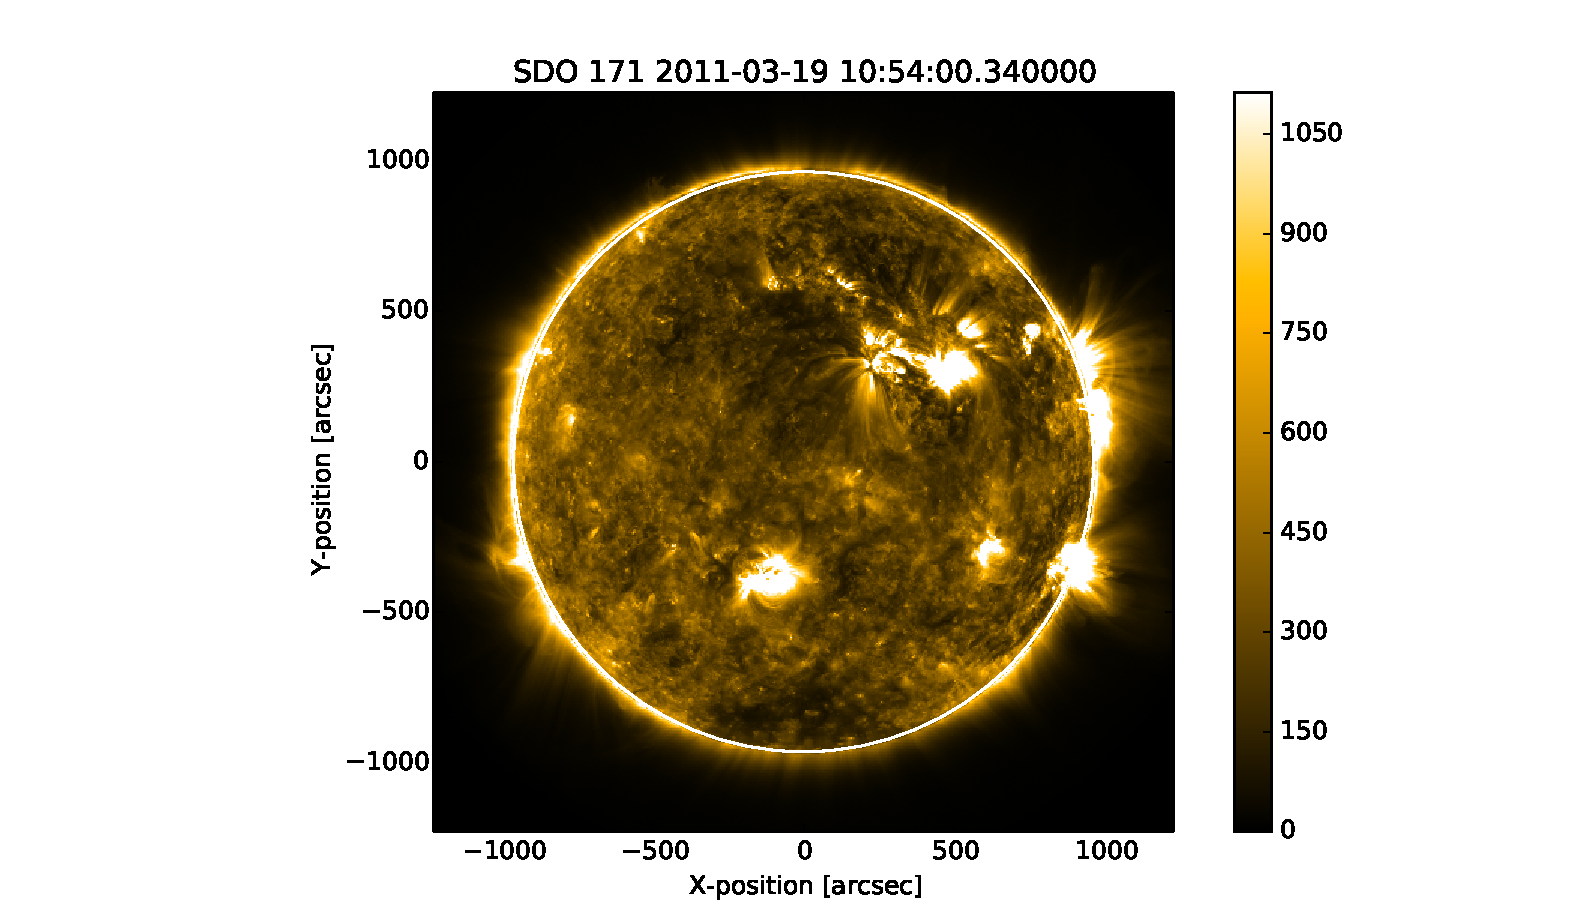
\includegraphics[width=0.8\columnwidth]{aia_map_example}
\end{center}
\caption{Example of the \texttt{AIAMap} specialisation of 
\texttt{GenericMap}. The map is created from an \textit{SDO}/AIA FITS file, a cutout
of the map is created, and then a quick-view plot is created with lines of heliographic longitude and latitude over-plotted.}
\label{code:aia_1}
\end{listing}

In addition to the data-type classes, the \texttt{map} subpackage provides two 
collection classes, \texttt{CompositeMap} and \texttt{MapCube}, for 
temporally and spatially aligned data respectively.
\texttt{CompositeMap} provides methods for overlaying spatially aligned 
data, with support for visualisation of images and contour lines overlaid 
upon each other.
\texttt{MapCube} provides methods for animation of its series of \texttt{Map} 
objects. Listings~\ref{code:compmap_1} and \ref{code:mapcube_1} show how to 
interact with these classes.

\begin{listing}[H]
\begin{minted}[bgcolor=bg]{pycon}
>>> import sunpy.map
>>> import matplotlib.pyplot as plt
>>> compmap = sunpy.map.Map('aia_1600_image.fits', 'RHESSI_image.fits', 
...                         composite=True)
>>> compmap.set_levels(1, range(0,50,5), percent=True)
>>> compmap.set_colors(1, 'Reds_r')
#Plot the result and crop
>>> ax = plt.subplot()
>>> compmap.plot()
>>> ax.axis([200, 600, -600, -200])
>>> plt.show()
\end{minted}
\begin{center}
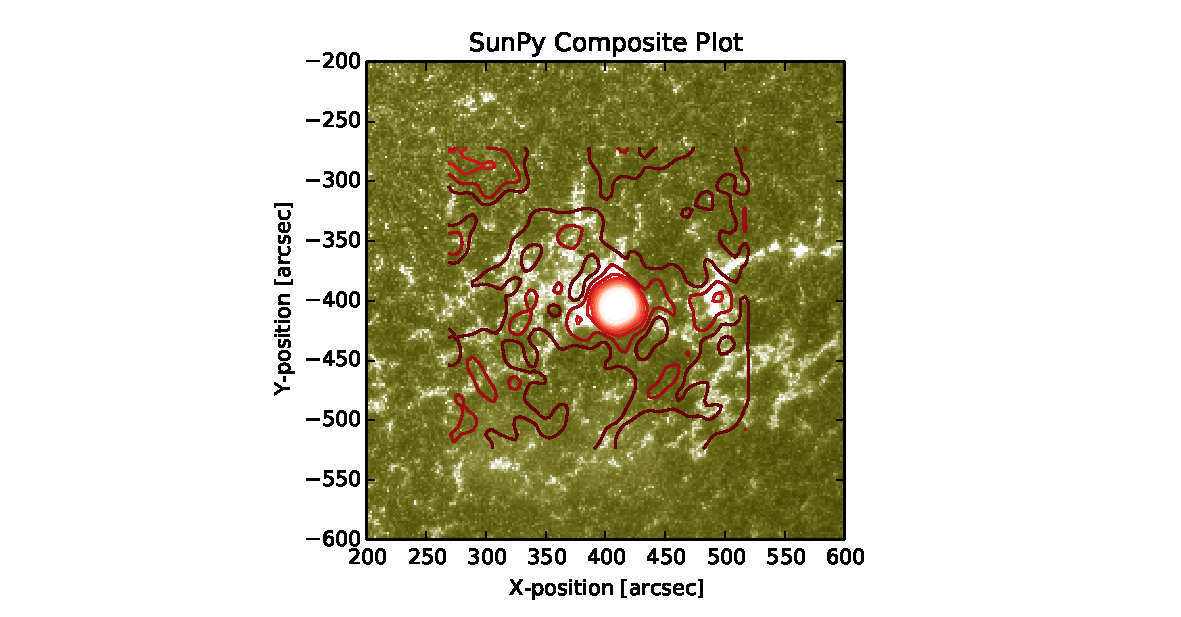
\includegraphics[width=0.8\columnwidth]{comp_map_example}
\end{center}
\caption{Example showing a \texttt{CompositeMap} plot, with RHESSI data composited
with \textit{SDO}/AIA data, and the integration with the \texttt{matplotlib.pyplot} interface.}
\label{code:compmap_1}
\end{listing}

\begin{listing}[H]
\begin{minted}[bgcolor=bg]{pycon}
>>> import sunpy.map
>>> cubemap = sunpy.map.Map('aia_lev1_171a_2014_01*fits', cube=True)
>>> cubemap.peek()
\end{minted}
\begin{center}
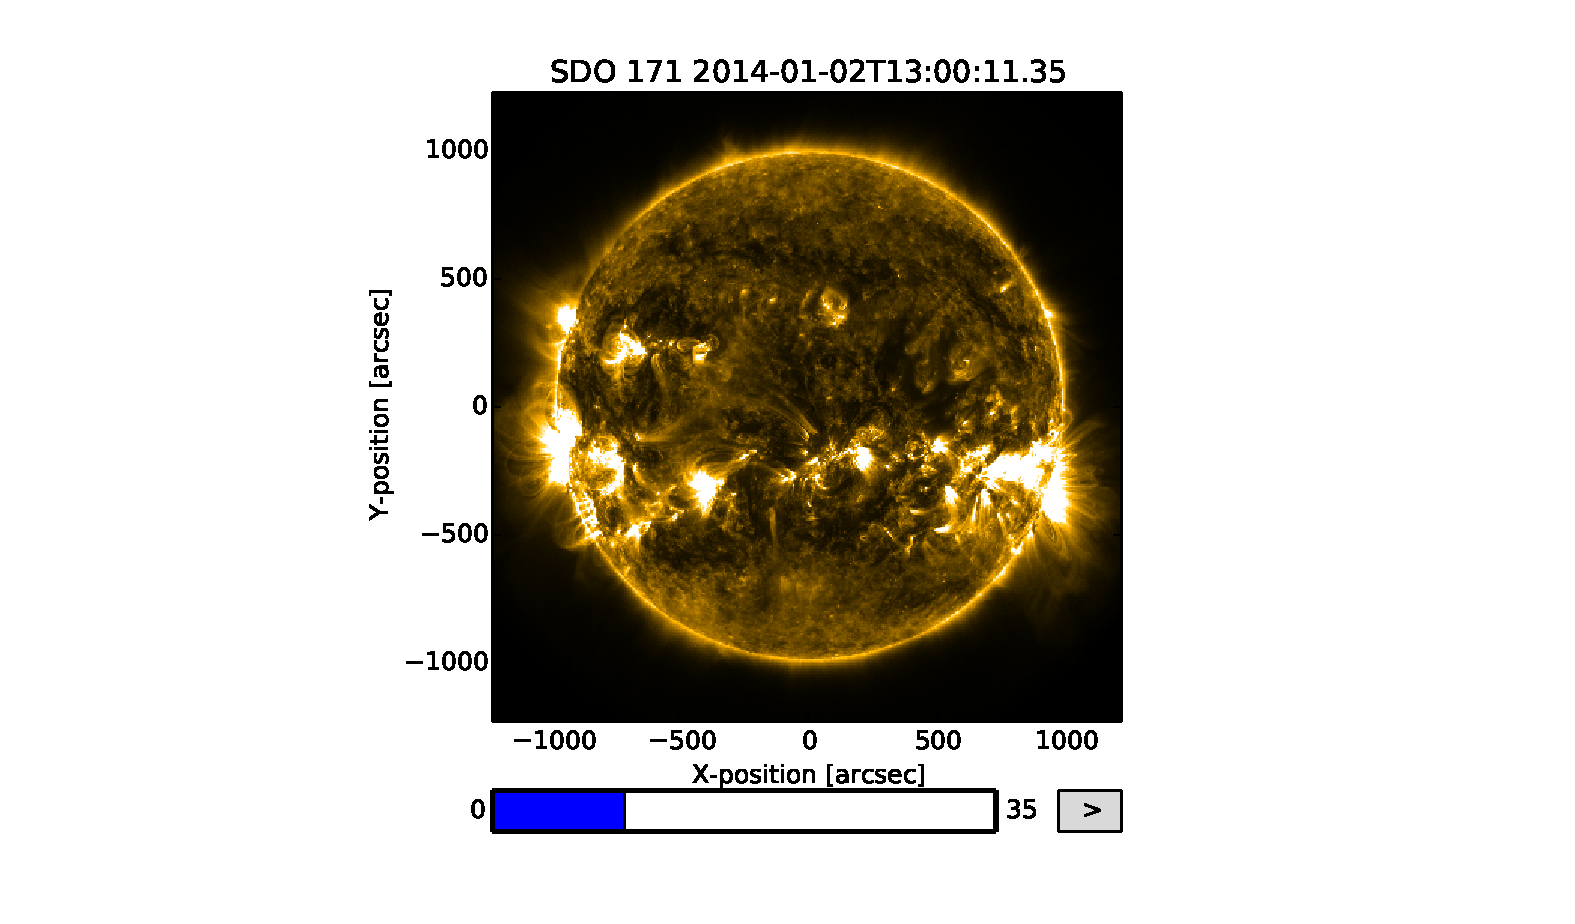
\includegraphics[width=0.8\columnwidth]{aia_cube_controls}
\end{center}
\caption{Example showing creation of a \texttt{MapCube} from a glob file search. The 
resultant plot makes use of \texttt{matplotlib}'s interactive widgets to allow scrolling 
through the \texttt{MapCube}.}
\label{code:mapcube_1}
\end{listing}
\subsection{Lightcurve}\label{ssec:lightcurve}

Time series data and their analyses are a fundamental aspect of solar
physics for which many data sources are available.
SunPy provides a \texttt{LightCurve} class
with a convenient and consistent interface for handling solar time-series
data.  The main engine behind the \texttt{LightCurve} class is
the {\texttt{pandas}} data-analysis library (\url{http://pandas.pydata.org}), and 
\texttt{LightCurve}'s \texttt{data} attribute is a \texttt{pandas.DataFrame} 
object.
The \texttt{pandas} library contains a large amount
of functionality for manipulating and analysing time-series data,
making it an ideal basis for \texttt{LightCurve}.  \texttt{LightCurve}
assumes that the input data are time-ordered list(s) of numbers, and each
list becomes a column in the \texttt{pandas} DataFrame object.

Currently, the \texttt{LightCurve} class is compatible with the
following data sources: the \textit{GOES} X-ray Sensor (XRS), \textit{PROBA2}/LYRA, and
the \textit{SDO} EUV Variability Experiment (EVE; only the level ``OCS'' and
% Do we need to explain what OCS means?
% RJH: I'd argue that everything other than (EVE) can be cut, but I'm not 
% confident enough to make that cut.
% dps: I agree, JI, what do you think?
average CSV files -- see \url{http://lasp.colorado.edu/home/eve/data/}
for more detail).  For each of these instruments, a subclass of the
\texttt{LightCurve} object is initialised
(e.g., \texttt{GOESLightCurve}) which inherits from
\texttt{LightCurve} but allows instrument-specific functionality to be
included.  Future developments will introduce support for additional
instruments and data products, as well as implementing a factory interface 
similar to that of \texttt{Map}.  Since there is no established standard
as to how time-series data should be stored and distributed, each SunPy 
\texttt{LightCurve} object sub-class provides the ability to download its corresponding 
specific data format in its constructor and parse that file type.

A \texttt{LightCurve} object may be created using a number of different methods. 
For example, a \texttt{LightCurve} may be created for a specific instrument given
an input time range. In Listing~\ref{code:goes_lc}, 
the \texttt{LightCurve} constructor searches a remote source for the GOES X-ray 
data specified by the time interval, downloads the required files and 
subsequently creates and plots the object.

%removed the resample part of the example - really we need to fix truncate!
% schriste - i think it would be better to show off some of the powerful pandas methods in this section
% as we are not likely to fix truncate and i think it should be refactored anyway
%ays: moved these comments outside of the listing in case we forget to delete these
\begin{listing}[H]
\begin{minted}[bgcolor=bg]{pycon}
>>> from sunpy import lightcurve
>>> from sunpy.time import TimeRange
>>> goes = lightcurve.GOESLightCurve.create('2011-06-07 06:00',
...                                         '2011-06-07 08:00')
>>> goes.peek()
\end{minted}
\begin{center}
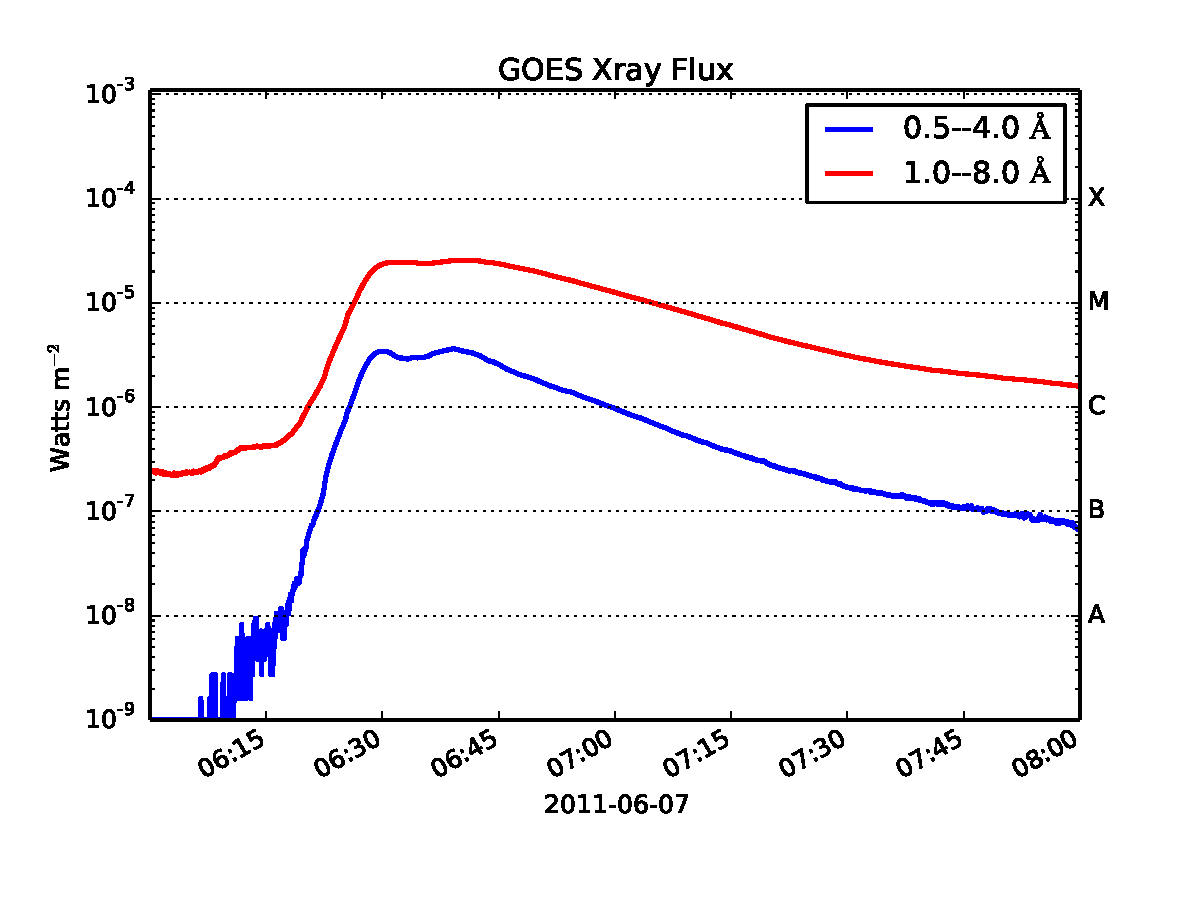
\includegraphics[width=10cm]{goes_lightcurve.pdf}
\end{center}
\caption{Example retrieval of a GOES lightcurve
using a time range, and the output of the 
\texttt{peek()} method.}
\label{code:goes_lc}
\end{listing}
%schriste - note to self, fix this example, add resampled points on top of plot?

Alternatively, if the data file already exists on the local system, the 
\texttt{Lightcurve} object may instead be initialised using that file as input.
Once the \texttt{Lightcurve} has been created, it may be manipulated in 
a variety of ways in order to perform time-series analysis.
%Stuart: Where did the pandas section go?
%ARI - looks like it's up top


\subsection{Spectra}\label{sec:spectra}
%schriste - this section needs major work
%ji - there is no example of a spectrum
%dps - I need to think in one...
%schriste - can't we just take a slice off of the spectram to make a spectrum?

SunPy aims to provide broad support for solar spectroscopy
instruments.  The variety and complexity of these instruments and
their resultant datasets makes this a challenging goal.  The \texttt{spectra} module implements a
\texttt{Spectrum} class for 1D data (intensity as a function of frequency) and a
\texttt{Spectrogram} class for 2D data (intensity as a function of time and
frequency).  Each of these classes use a \texttt{numpy.ndarray} class
as its \texttt{data} attribute.  These two classes were implemented
by funding provided by the Astrophysics Research Group at Trinity
College Dublin, Ireland.

As with other SunPy data types, the \texttt{Spectrogram} class has been
built so that each instrument initialises using a subclass containing the instrument-specific 
functionalities. The common functionality provided by the base \texttt{Spectrogram} class includes
joining different time ranges and frequencies, performing frequency-dependent background subtraction,
and convenient visualization and sampling of the data.
Currently, the \texttt{Spectrogram} class supports radio spectrograms from the 
\href{http://www.e-callisto.org/}{e-Callisto}
solar radio spectrometer network and STEREO/SWAVES spectrograms.

Listing \ref{code:spectra} shows how the \texttt{CallistoSpectrogram}
object retrieves spectrogram data in the time range specified taken at
the observatory of interest.  When the data is requested using the
\texttt{from\_range()} function, the object merges all the downloaded
files into a single spectrogram, across time and frequency.
In the example shown, data is provided in two frequency ranges, 
20--90\,MHz and 55--355\,MHz.  Since the data is not evenly spaced in
the frequency range, the \texttt{Spectrogram} object linearises the
frequency axis for a better analysis.  The example also demonstrates
the implemented background subtraction method.
% RJH: Which subtraction method?  If the specifics are irrelevant, cut it.
%ji to DPS - what is the linearisation that is happening here?

\begin{listing}[H]
\begin{minted}[bgcolor=bg]{pycon}
>>> from sunpy.spectra.sources.callisto import CallistoSpectrogram
>>> tstart, tend = "2011-06-07T06:00:00", "2011-06-07T07:45:00"
>>> callisto = CallistoSpectrogram.from_range("BIR", tstart, tend)
>>> callisto_nobg = callisto.subtract_bg()
>>> callisto_nobg.peek(vmin = 0)
\end{minted}
\begin{center}
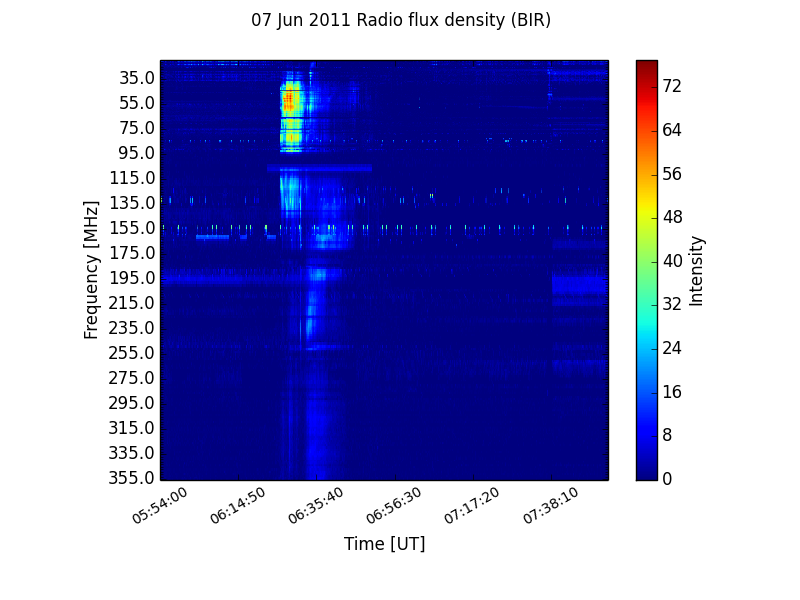
\includegraphics[width=0.8\columnwidth]{callisto_nobg}
\end{center}
\caption{Example of how \texttt{CallistoSpectrogram} retrieves the
  data for the requested time range and observatory, merges it and
  removes the background signal.  The data requested -- `BIR' -- is
  the code name of the \href{http://www.rosseobservatory.ie}{Rosse Observatory}
  at Birr Castle in Ireland.}
\label{code:spectra}
\end{listing}

% Download Callisto
% Merge multiple time-ranges / frequencies (just work from downlad!)
% Merge callisto with swaves



\subsection{Visualisation}
\label{subsec:Viz}
As demonstrated in this section, the core SunPy datatypes 
include visualisation methods that are tailored to that data type. 
These visualisation methods all currently utilise the \texttt{matplotlib} 
package, and are designed in such a way that they integrate well with 
the \texttt{pyplot} functional interface of \texttt{matplotlib}.

This design philosophy makes the behaviour of SunPy's visualisation 
routines intuitive to those who already understand the \texttt{matplotlib}
interface, as well as allowing the use of the standard 
\texttt{matplotlib} commands to manipulate the plot parameters (e.g. title, axes).